\documentclass[aspectratio=169]{beamer}

\mode<presentation>

\usepackage[utf8]{inputenc}
\usepackage[T1]{fontenc}	%makes å,ä,ö etc. proper symbols
\usepackage{amsmath}
\usepackage{graphicx}
\usepackage{xcolor}
\usepackage{listings}
\usepackage{multicol}
\usepackage{hyperref}
\usepackage[swedish]{babel}

\definecolor{LundaGroen}{RGB}{00,68,71}
\definecolor{StabilaLila}{RGB}{85,19,78}
\definecolor{VarmOrange}{RGB}{237,104,63}

\definecolor{MagnoliaRosa}{RGB}{251,214,209}
\definecolor{LundaHimmel}{RGB}{204,225,225}
\definecolor{LundaLjus}{RGB}{255,242,191}

\usefonttheme{serif}
\usetheme{malmoe}
\setbeamercolor{palette primary}{bg=LundaHimmel, fg=StabilaLila}
\setbeamercolor{palette quaternary}{bg=LundaGroen, fg=MagnoliaRosa}
\setbeamercolor{background canvas}{bg=LundaLjus}
\setbeamercolor{structure}{fg=LundaGroen}

\usepackage[many]{tcolorbox}

\newtcolorbox{cross}{blank,breakable,parbox=false,
  overlay={\draw[red,line width=5pt] (interior.south west)--(interior.north east);
    \draw[red,line width=5pt] (interior.north west)--(interior.south east);}}
    
\newcommand{\code}[1]{\colorbox{white}{\lstinline{#1}}}



\lstset{language=Python} 
\lstset{%language=[LaTeX]Tex,%C++,
    morekeywords={PassOptionsToPackage,selectlanguage,True,False},
    keywordstyle=\color{blue},%\bfseries,
    basicstyle=\small\ttfamily,
    %identifierstyle=\color{NavyBlue},
    commentstyle=\color{red}\ttfamily,
    stringstyle=\color{VarmOrange},
    numbers=left,%
    numberstyle=\scriptsize,%\tiny
    stepnumber=1,
    numbersep=8pt,
    showstringspaces=false,
    breaklines=true,
    %frameround=ftff,
    frame=single,
    belowcaptionskip=.75\baselineskip,
	tabsize=4,
	backgroundcolor=\color{white}
    %frame=L
}
\lstset{
	escapeinside={(*@}{@*)}
}
\begin{document}

\lstset{literate=
  {á}{{\'a}}1 {é}{{\'e}}1 {í}{{\'i}}1 {ó}{{\'o}}1 {ú}{{\'u}}1
  {Á}{{\'A}}1 {É}{{\'E}}1 {Í}{{\'I}}1 {Ó}{{\'O}}1 {Ú}{{\'U}}1
  {à}{{\`a}}1 {è}{{\`e}}1 {ì}{{\`i}}1 {ò}{{\`o}}1 {ù}{{\`u}}1
  {À}{{\`A}}1 {È}{{\'E}}1 {Ì}{{\`I}}1 {Ò}{{\`O}}1 {Ù}{{\`U}}1
  {ä}{{\"a}}1 {ë}{{\"e}}1 {ï}{{\"i}}1 {ö}{{\"o}}1 {ü}{{\"u}}1
  {Ä}{{\"A}}1 {Ë}{{\"E}}1 {Ï}{{\"I}}1 {Ö}{{\"O}}1 {Ü}{{\"U}}1
  {â}{{\^a}}1 {ê}{{\^e}}1 {î}{{\^i}}1 {ô}{{\^o}}1 {û}{{\^u}}1
  {Â}{{\^A}}1 {Ê}{{\^E}}1 {Î}{{\^I}}1 {Ô}{{\^O}}1 {Û}{{\^U}}1
  {œ}{{\oe}}1 {Œ}{{\OE}}1 {æ}{{\ae}}1 {Æ}{{\AE}}1 {ß}{{\ss}}1
  {ű}{{\H{u}}}1 {Ű}{{\H{U}}}1 {ő}{{\H{o}}}1 {Ő}{{\H{O}}}1
  {ç}{{\c c}}1 {Ç}{{\c C}}1 {ø}{{\o}}1 {å}{{\r a}}1 {Å}{{\r A}}1
  {€}{{\euro}}1 {£}{{\pounds}}1 {«}{{\guillemotleft}}1
  {»}{{\guillemotright}}1 {ñ}{{\~n}}1 {Ñ}{{\~N}}1 {¿}{{?`}}1
}

% NEW COMMANDS
\newcommand{\fortt}{\texttt{for}}
\newcommand{\whilett}{\texttt{while}}
\newcommand{\iftt}{\texttt{if}}

\AtBeginSection[ ]
{
\begin{frame}{Outline}
    \tableofcontents[currentsection]
\end{frame}
}

\title{Stackar}
\date{vt 25}
\author{Programmering 2}

\maketitle

\tableofcontents

\section{Stackar}

\subsection{Vad är en stack?}

\begin{frame}
	\frametitle{Stackar}
	
	En \textit{stack} är en datastruktur där varje element refererar till ett annat element. De påminner lite granda om listor, med skillnaden att man brukar inte kunna komma åt valfria element, utan enbart det sista elementet i \textit{stacken}.
	
\end{frame}

\begin{frame}
	\frametitle{Exempel}
	
	En vanlig \textit{stack} IRL är en korthög. I flera kortspel så delar man ut ett antal kort till spelarna och sen lägger man resterande kort i en hög. Under spelets gång så drar man sedan det översta -- och alltid det översta -- kortet ur högen. När kortet är draget så försvinner det ur högen och nästa kort ligger överst.
	
\end{frame}

\subsection{LIFO}

\begin{frame}
	\frametitle{Stackar}
	\framesubtitle{Last In First Out}
	
	En \textit{stack} fungerar efter samma princip som anställningar på en större arbetsplats med ''Last In First Out'', LIFO. Alltså att det element, eller den anställd, som tillkom senast är det element som kommer plockas bort först när man plockar bort något --- alltså att den senast anställda är den som sägs upp först.

\end{frame}

\subsection{Metoder}

\begin{frame}
	\frametitle{Stackar}
	
	En \textit{stack} har följande tre metoder:
	
	\begin{enumerate}
		\item push
		\item peek			
		\item pop
	\end{enumerate}
	
\end{frame}


\begin{frame}
	\frametitle{Metoder}
	
	\begin{itemize}[<+->]
		\item Metoden \texttt{push} lägger till ett element sist  (överst) i \textit{stacken}. Du kan jämföra det med metoden \texttt{append} i listor.
	
		\item Metoden \texttt{peek} tittar på det sista (översta) elementet i \textit{stacken} och ger värdet.
	
		\item Metoden \texttt{pop} plockar bort det sista (översta), värdet i \textit{stacken}. Du kan jämföra det med motsvarande metod i listor.
		
	\end{itemize}
	
\end{frame}


\section{Stackar och listor}

\subsection{Listor som stackar}

\begin{frame}[fragile]
	\frametitle{Listor som stackar}
	\framesubtitle{Listor}

	I Python kan du simulera en \textit{stack} med en lista. Det är ganska ganska enkelt eftersom listan har alla metoder en \textit{stack} har och lite till.
	
	\begin{lstlisting}
stack = []
stack.append(4) # Motsvarar push
stack[-1] # Motsvarar peek
stack.pop() # Motsvarar pop
	\end{lstlisting}
	
\end{frame}
	
\subsection{Nackdelen med listor}
	
\begin{frame}
	\frametitle{Stackar och listor}
	\framesubtitle{Nackdelen med listor}
	
	Nackdelen med listor är att listor är en sammanhängande grupp i minnet på datorn. När man lägger till nya element i listan riskerar den att inte längre få plats på sin allokerade del i minnet, och då måste man flytta på HELA listan. Detta gör att operationer på listor kan ta olika lång tid att göra.

\end{frame}

\subsection{Fördelen med stackar}

\begin{frame}
	\frametitle{Stackar och listor}
	\framesubtitle{Fördelen med stackar}
	
	\textit{Stackar} däremot lagrar varje element separat i minnet, det kan ge lite mer overhead i varje element. Men det gör att man inte riskerar att flytta på hela \textit{stacken} när man lägger till element i den. Detta gör att operationer med \textit{stackar} är konsekventa i hur lång tid de tar att genomföra.
	
\end{frame}

\section{Övningar}

\subsection{Instruktioner och klassdiagram}

\begin{frame}[fragile]
	\frametitle{Övningar}
	\framesubtitle{Sida 1, Node}
	
	Följ pseudokod på följande slides (totalt 4) och skapa en \texttt{Stack} bestående av \texttt{Noder}. Skriv din kod i filen \texttt{stacks.py} (finns på Vklass) som har en \textit{driver code} som testar dina klasser.
	
	Här ser du klassdiagramen för dem två klasserna
	
	\begin{center}
		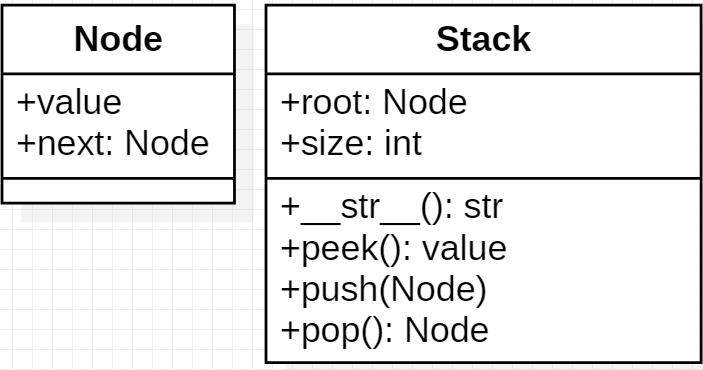
\includegraphics[width=.5\textwidth]{stackuml.png}
	\end{center}
	
\end{frame}

\subsection{Node}

\begin{frame}[fragile]
	\frametitle{Övningar}
	\framesubtitle{Sida 1, Node}
	
	\begin{lstlisting}
CLASS Node:
    METHOD __init__ takes in parameter value:
        SET self.value to value
        SET self.next to None
	\end{lstlisting}

\end{frame}

\subsection{Stack: init + \_\_str\_\_}

\begin{frame}[fragile]
	\frametitle{Övningar}
	\framesubtitle{Sida 2, Stack}
	
	\begin{lstlisting}
CLASS Stack:
    METHOD __init__:
        SET self.root to Node('root')
        SET self.size to 0
        
    METHOD __str__:
        SET out_string to ""
        SET current to self.root.next
        WHILE current:
            SET out_string to out_string + str(current.value) + '->'
            SET current to current.next
        RETRUN out_string[:-2]
	\end{lstlisting}
	
\end{frame}

\subsection{Stack: peek + push}

\begin{frame}[fragile]
	\frametitle{Övningar}
	\framesubtitle{Sida 3, Stack}
	
	\begin{lstlisting}
    METHOD peek:
        IF self.size is 0:
            RAISE Exception
        RETURN self.root.next.value
        
    METHOD push takes in parameter value:
        SET node to Node(value)
        SET node.next to self.root.next
        SET self.root.next to node
        SET self.size to self.size + 1
	\end{lstlisting}
	
\end{frame}

\subsection{Stack: pop}

\begin{frame}[fragile]
	\frametitle{Övningar}
	\framesubtitle{Sida 4, Stack}
	
	\begin{lstlisting}
    METHOD pop:
        IF self.size is 0:
            RAISE Exception
        SET remove to self.root.next
        SET self.root.next to remove.next
        SET self.size to self.size - 1
        RETURN remove.value
	\end{lstlisting}
	
\end{frame}

\end{document}